%%%%%%%%%%%%%%%%%%%%%%%%%%%%%%%%%%%%%%%%%%%%%%%%%%%%%%%%%%%%%%%%%%%%%%
%%% Stability analysis for angle modes %%%%%%%%%%%%%%%%%%%%%%%%%%%%%%%
%%%%%%%%%%%%%%%%%%%%%%%%%%%%%%%%%%%%%%%%%%%%%%%%%%%%%%%%%%%%%%%%%%%%%%
\documentclass[twocolumn,prd,showpacs,
%nobalancelastpage,
floatfix,preprintnumbers,nofootinbib]{revtex4}

\usepackage{epsfig}
\usepackage{amsmath,bm}

\newcommand{\I}{{\rm i}}

\graphicspath{{./figs/}}
%%%%%%%%%%%%%%%%%%%%%%%%%%%%%%%%%%%%%%%%%%%%%%%%%%%%%%%%%%%%%%%%%%%%%

\begin{document}

\title{Flavor instability in dense neutrino streams caused by
discrete angle distributions}

\author{Srdjan Sarikas, David Seixas and Georg Raffelt}
\affiliation{Max-Planck-Institut f\"ur Physik
(Werner-Heisenberg-Institut), F\"ohringer Ring 6, 80805 M\"unchen,
Germany}

\date{\today}

%%%%%%%%%%%%%%%%%%%%%%%%%%%%%%%%%%%%%%%%%%%%%%%%%%%%%%%%%%%%%%%%%%%

\begin{abstract}
The dense neutrino flux streaming from a core-collapse supernova can
undergo self-induced flavor conversion caused by neutrino-neutrino
refraction. In numerical studies, the neutrino radiation field is
represented by discrete energy and angle bins. The former can be
chosen according to the desired spectral resolution. On the other
hand, if the number of angle bins $N_a$ is chosen too small,
completely unphysical solutions arise, e.g.\ flavor conversion
begins at a spurious depth and then usually causes kinematical
decoherence. On the other hand, $N_a=1$ (single-angle approximation)
can be a good proxy for the $N_a\to\infty$ limit. Based on a
linearized stability analysis, we explain the puzzling $N_a$
dependence.
\end{abstract}


\preprint{MPP-2012-XXX}

\pacs{14.60.Pq, 97.60.Bw}

\maketitle


%%%%%%%%%%%%%%%%%%%%%%%%%%%%%%%%%%%%%%%%%%%%%%%%%%%%%%%%%%%%%%%%%%%%%%
\section{Introduction}
\label{sec:intro}
%%%%%%%%%%%%%%%%%%%%%%%%%%%%%%%%%%%%%%%%%%%%%%%%%%%%%%%%%%%%%%%%%%%%%%

The huge flux of neutrinos emitted from a collapsed supernova (SN)
core begins to stream almost freely at a radius of 10--30~km,
depending on the explosion phase and the neutrino energies, and at a
density of some $10^{12\hbox{--}13}~{\rm g}/{\rm cm}^3$. For such
conditions, neutrino refraction by matter is so large that
propagation eigenstates are almost identical with weak interaction
eigenstates even though all neutrino mixing angles are relatively large.
Despite this simple boundary condition, the subsequent neutrino
flavor evolution is surprisingly complicated due to the nonlinear
impact of neutrino-neutrino refraction~\cite{Duan:2006an,
Duan:2010bg}.

Main problem in understanding this phenomenon is that numerical
studies of the flavor evolution are challenging. If the integration
begins close to the neutrino sphere, large oscillation frequencies
caused by the large matter effect require many time steps. Moreover,
the neutrino radiation field must be represented in some numerical
form, in practice a finite number of energy and angle bins. Thus far
axial symmetry of the neutrino stream was always assumed, implying
that there was only one angle variable. Even with this
simplification, reliable results require a large-scale computing
effort~\cite{Duan:2008eb}.

Far away from the SN core, for example at a detector on Earth, we do
not care about the angle distribution and good energy resolution
would be enough. In particular, self-induced flavor conversion can
lead to sharp spectral features that one wants to
resolve~\cite{Duan:2006an, Raffelt:2007cb, Duan:2007fw,
Fogli:2007bk, Dasgupta:2009mg}. Many studies therefore used the
single-angle approximation where all neutrinos are represented by a
single angle bin, e.g.\ emission at $45^\circ$ relative to the
radial direction. The simplest assumption of radially emitted
neutrinos is not possible because parallel-moving neutrinos do not
provide a refractive effect for each other.

To improve on single-angle studies, a small number $N_a$ of angle bins 
is not enough. Beginning with the earliest studies~\cite{Duan:2006an}, 
everybody trying multi-angle simulations has been spooked by the same 
curious effect. Although high number of angular bins ($N_a\to\infty$) 
and single-angle solutions tend to provide similar results, if $N_a$ is 
``small'', the results would be completely different from the two 
limiting cases. The required $N_a$ has
completely eluded explanation. Depending on circumstances, a few
tens of modes can be enough, but in other cases one needs thousands
or more. \marginpar{\tiny Another approach is to avoid angular bins and expand the
radiation field in spherical harmonics, but the required multipole
order is just as large~\cite{Raffelt:2007yz}.}

For a simple (``single-crossed'' \cite{Dasgupta:2009mg}) neutrino
spectrum, relevant during the SN accretion phase, self-induced
flavor conversion begins at a critical onset radius.
If only neutrino-neutrino refraction is relevant\footnote{For now we ignore refraction by matter and the ``multi-angle matter effect'' which can suppress self-induced flavor conversion~\cite{Raffelt:2008hr, Duan:2010bf, EstebanPretel:2008ni, Chakraborty:2011gd, Sarikas:2011am}.}, then at larger neutrino
density, close to the SN core, the system is stable (``sleeping top'' phase
\cite{Hannestad:2006nj, Duan:2007mv}). The onset radius is almost
the same in the single-angle and many-mode limits. On the other
hand, if $N_a>1$ is too small, flavor conversion begins at a smaller
radius (higher neutrino densities) and tends to cause kinematical decoherence among angle modes~\cite{EstebanPretel:2007ec}.

This few-mode flavor conversion effect must begin with an
instability, i.e.\ with a run-away flavor mode in the interacting
neutrino system. Understanding self-induced flavor conversion based
on a linearized stability analysis was pioneered by
Sawyer~\cite{Sawyer:2008zs} and further developed by our group and
collaborators~\cite{Banerjee:2011fj, Sarikas:2011am}. We here apply
this technique to the \hbox{``$N_a$ effect''} and find that many
puzzling numerical observations easily fall into place. The spectrum
of run-away modes is indeed very different for ``$N_a={}$few'' from
$N_a=1$ and $N_a\to\infty$. The two neutrino mass hierarchies show
striking differences.

This situation is to be contrasted with the role of energy bins that
can be chosen to the desired resolution without affecting the
qualitative behavior. Collective flavor motion is here described by
a small number of collective variables (``$N$-mode coherence''),
independently of the number of energy bins \cite{Raffelt:2010za,
Raffelt:2011yb, Yuzbashyan:2008}. We can therefore study conceptual
multi-angle effects in the single-energy approximation where we use
only one energy bin for neutrinos and one for anti-neutrinos.


\clearpage

%%%%%%%%%%%%%%%%%%%%%%%%%%%%%%%%%%%%%%%%%%%%%%%%%%%%%%%%%%%%%%%%%%%%%%
\section{Linearized stability approach}
\label{sec:linearized}
%%%%%%%%%%%%%%%%%%%%%%%%%%%%%%%%%%%%%%%%%%%%%%%%%%%%%%%%%%%%%%%%%%%%%%

\subsection{Equations of motion}

Following earlier works~\cite{EstebanPretel:2008ni, Banerjee:2011fj,
Sarikas:2011am}, we describe the two-flavor neutrino field by
energy- and angle-dependent $2{\times}2$ matrices
${\bf\Phi}_{E,u}(r)$. Boldface characters denote matrices in flavor
space. The diagonal ${\bf\Phi}_{E,u}$ elements are the ordinary
number fluxes $F_{E,u}^\alpha$ (flavor $\alpha$) integrated over a
sphere of radius $r$, with negative $E$ for anti-neutrinos.
Moreover, we use the ``flavor isospin convention'' where
$F_{E,u}^\alpha<0$ for antineutrinos ($E<0$) and $F_{E,u}^\alpha>0$
for neutrinos ($E>0$). 

The off-diagonal elements of ${\bf\Phi}_{E,u}(r)$, which are
initially very small, represent phase information caused by flavor
oscillations. The flavor evolution follows from the
Schr\"odinger-like equation \cite{EstebanPretel:2008ni}
\begin{equation}
{\rm i}\partial_r{\bf\Phi}_{E,u}=[{\bf H}_{E,u},{\bf\Phi}_{E,u}]
\end{equation}
with the Hamiltonian
\begin{eqnarray}\label{eq:hamiltonian}
{\bf H}_{E,u}&=&\frac{1}{v_{u}}\,\left(\frac{{\bf M}^2}{2E}+
\sqrt{2}\,G_{\rm F}{\bf N}_\ell\right)\\
&+&\frac{\sqrt{2}\,G_{\rm F}}{4\pi r^2}\int_{-\infty}^{+\infty}dE'
\int_0^1 du'
\frac{1-v_{u}v_{u'}}{v_{u}v_{u'}}\,{\bf\Phi}_{E',u'}\,.
\nonumber
\end{eqnarray}
The matrix ${\bf M}^2$ of neutrino mass-squares causes vacuum flavor
oscillations and that of net charged lepton densities ${\bf
N_\ell}={\rm diag}(n_e{-}n_{\bar
e},n_\mu{-}n_{\bar\mu},n_\tau{-}n_{\bar\tau})$ adds the matter
effect. The third term provides neutrino-neutrino refraction. A
neutrino radial velocity at radius $r$ is
$v_u=(1-u\,R^2/r^2)^{1/2}$, where the angular variable $u$ is defined in
terms of the angle $\theta_R$ at which the neutrino is emitted at some 
conveniently chosen radius $R$. The factor $1-v_u v_{u'}$ arises from
the current-current nature of the weak interaction and causes
multi-angle effects. Moreover, $v_u$ appears in the denominator
because we follow the flavor evolution projected on the radial
direction.

We study the instability driven by the atmospheric $\Delta m^2$ and
the mixing angle $\theta_{13}$. In the relevant SN region,
propagation eigenstates are almost identical with weak-interaction
eigenstates unless self-induced flavor conversion occurs. This means
that initially the off-diagonal elements of ${\bf\Phi}_{E,u}$ are
very small, justifying a linearized stability analysis, but
otherwise we do not need a specific numerical value of the mixing
angle.

We switch to the variable $\omega=\Delta m^2/2E$ which is much
better suited to flavor oscillation studies than energy itself.
Finally, we write the flux matrices in the form
\begin{equation}
{\bf\Phi}_{\omega,u}=\frac{{\rm Tr}\,{\bf\Phi}_{\omega,u}}{2}
+\frac{F_{\omega,u}^e-F_{\omega,u}^x}{2}\,
\begin{pmatrix}
s_{\omega,u}&S_{\omega,u}\\
S_{\omega,u}^*&-s_{\omega,u}
\end{pmatrix}\,,
\end{equation}
where $F_{\omega,u}^{e,x}$ are the flavor fluxes at the inner
boundary radius $R$. The flux summed over all flavors, ${\rm
Tr}\,{\bf\Phi}_{\omega,u}$, is conserved in our free-streaming
limit. The $\nu_e$ survival probability is
$\frac{1}{2}[1+s_{\omega,u}(r)]$ in terms of the ``swap factor''
$-1\leq s_{\omega,u}(r)\leq1$. The off-diagonal element
$S_{\omega,u}$ is complex and $s^2_{\omega,u}+|S_{\omega,u}|^2=1$.


\subsection{Stability condition}

The possible onset of self-induced flavor conversions is best
described in terms of the complex numbers $S_{\omega,u}$ which are
very small as long as neutrinos are in weak interaction eigenstates
in the presence of matter. The small-amplitude limit means
$|S_{\omega,u}|\ll1$ and to linear order $s_{\omega,u}=1$. Assuming
in addition a large distance from the source so that $1-v_u\ll 1$,
the evolution equation linearized in $S_{\omega,u}$ and in $u$ is
\cite{Banerjee:2011fj}
\begin{eqnarray}\label{eq:smallEoM}
{\rm i}\partial_r S_{\omega,u}&=&
(\omega + u\bar\lambda)\,S_{\omega,u}
\nonumber\\
& &-\mu \int du'\,d\omega'\,(u+u')\,g_{\omega'u'}\,S_{\omega',u'}\,.
\label{stability-eom}
\end{eqnarray}
Here, $g_{\omega,u}$ is the neutrino spectrum ($\omega<0$
antineutrinos) which we normalize to the anti-neutrino flux, i.e.\
$\int_{-\infty}^0 d\omega\int_0^1 du\,g_{\omega,u}=-1$. The
``asymmetry'' between neutrinos and antineutrinos is
$\varepsilon=\int d\omega\, du\,g_{\omega,u}$.

Refractive effects are encoded in the $r$-dependent parameters
\begin{eqnarray}
\lambda&=&\sqrt{2}\,G_{\rm F}\,[n_e(r)-n_{\bar e}(r)]\,\frac{R^2}{2r^2}\,,
\nonumber\\
\mu&=&\frac{\sqrt{2}\,G_{\rm F}\,[F_{\bar\nu_e}(R)-F_{\bar\nu_x}(R)]}{4\pi r^2}
\,\frac{R^2}{2r^2}\,,
\end{eqnarray}
and often combined in $\bar{\lambda} = \lambda + \epsilon\mu$.
The factor $R^2/2r^2$ signifies that only the multi-angle impact of
the $\nu$-$\nu$ and matter effects are relevant for the stability
analysis, not the densities themselves. Our normalizations are such
that the neutrino-neutrino interaction strength $\mu$ is normalized
to the $\bar\nu_e$-$\bar\nu_x$ flux difference at a chosen radius
$R$, the nominal neutrino sphere. Physical results do not depend on
the choice of $R$.

Writing solutions of the linear differential equation,
Eq.~(\ref{eq:smallEoM}), in the form
\begin{equation}
S_{\omega,u}=Q_{\omega,u}\,e^{-{\rm i}\Omega r}
\end{equation}
with complex frequency $\Omega=\gamma+{\rm i}\kappa$ and eigenvector
$Q_{\omega,u}$ leads to the eigenvalue
equation~\cite{Banerjee:2011fj},
\begin{equation}\label{fourier-eom}
(\omega + u\bar\lambda - \Omega)\, Q_{\omega,u}=
\mu \int du'\,d\omega'\,(u+u')\,g_{\omega'u'}\,Q_{\omega',u'}\,.
\end{equation}
Following Ref.~\cite{Banerjee:2011fj} we note that both sides of
this equation are a linear polynomial in $u$, implying
\begin{equation}
Q_{\omega,u}=\frac{a+bu}{\omega+u\bar\lambda-\Omega}\,.
\end{equation}
For fixed $\omega$, the numbers $Q_{\omega,u}$ as a function of
$0\leq u\leq1$ lie on a circular arc in the complex plane and
likewise, for fixed $u$, the $Q_{\omega,u}$ as a function of
$-\infty<\omega<+\infty$ form a circle. 

Self-consistency requires that
\begin{equation}\label{eq:abmatrix}
\begin{pmatrix} I_1-1&I_2\\ I_0&I_1-1\end{pmatrix}
\begin{pmatrix} a\\ b\end{pmatrix}=0\,,
\end{equation}
where
\begin{equation}
I_n=\int du\,d\omega\,
\frac{u^n\mu\,g_{\omega,u}}{\omega+u\bar\lambda-\Omega}\,.
\label{eq:In-def}
\end{equation}
In contrast with Ref.~\cite{Banerjee:2011fj} we have included a
factor $\mu$ in the integral to make $I_n$ dimensionless.

Nontrivial solution for $a$ and $b$ exist if the determinant of the
matrix in Eq.~(\ref{eq:abmatrix}) vanishes, implying
\begin{equation}\label{eq:multiangleeigenvalue}
(I_1-1)^2=I_0 I_2\, .
\end{equation}
A change in the hierarchy amounts to the exchange of sign of the mass matrix  $\bf M$ in 
Eq.~(\ref{eq:hamiltonian}), which results in the sign change 
$\omega\to-\omega$ only in the denominator of the integrand in 
Eq.~\ref{eq:In-def}. In the remaining text, inverted hierarchy will be 
assumed if not explicitly stated.

%\subsection{Single angle}

%In the single-angle approach one assumes that the spectrum is of the
%form
%\begin{equation}
%g_{\omega,u}=g_\omega\,\delta(u-u_1)\,.
%\end{equation}
%Since we are primarily interested in the imaginary part of $\Omega$,
%we can go to a rotating frame by the substitution
%$\Omega\to\Omega-u_1\bar\lambda$. One then easily finds the
%self-consistency condition from Eq.~(\ref{fourier-eom}) with the
%ansatz $Q_\omega\propto(\omega-\Omega)^{-1}$
%\begin{equation}
%h=2u_1\int_{-\infty}^{+\infty}d\omega\,\frac{\mu\,g_\omega}{\omega-\Omega}\,.
%\end{equation}
%One finds the same result starting from
%Eq.~(\ref{eq:multiangleeigenvalue}).

%%%%%%%%%%%%%%%%%%%%%%%%%%%%%%%%%%%%%%%%%%%%%%%%%%%%%%%%%%%%%%%%%%%%%%
\section{Continuum and Single Angle}
\label{sec:single angle}
%%%%%%%%%%%%%%%%%%%%%%%%%%%%%%%%%%%%%%%%%%%%%%%%%%%%%%%%%%%%%%%%%%%%%%

\subsection{Neutrino Spectrum}

We use the simplest nontrivial set-up that allows us to study the
role of discrete angle modes. We consider a neutrino flux streaming
from a sphere at radius $R$ that emits monochromatic fluxes of
$\bar\nu_e$ and $\nu_e$, the latter with a flux $1+\epsilon$ larger
than the former. 
The chosen vacuum frequency for neutrinos and antineutrinos $\pm\omega_0$ essentially determines the frequency scale of the system. We simplify the calculations by choosing $\omega_0=1$ as the unit of measure for all other frequencies ($\mu,\lambda,\kappa,\gamma$). When discussing the realistic SN situation we will use a more realistic value of $\omega_0 = 0.5~{\rm km}^{-1}$.

The angle distribution is taken to be black-body like, i.e.\ the
neutrino sphere is taken to emit neutrino isotropically into space
without limb darkening. This implies a box-spectrum in the $u$
variable of the form
\begin{equation}
B(u)=\begin{cases}1&\hbox{for $0\leq u\leq1$},\\
0&\hbox{otherwise.}\end{cases}
\end{equation}
Therefore, overall we study the neutrino spectrum
\begin{equation}
g_{\omega,u}=\Bigl[-\delta(-\omega_0-\omega)+
(1+\epsilon)\,\delta(\omega_0-\omega)\Bigr]\,B(u)\,.
\end{equation}

\subsection{Inverted Hierarchy}
%%%%%%%%%%%%%%%%%%%%%%%%%%%%%%%%%%%%%%%%%%%%%%%%%%%%%%%%%%%%%%%%
\begin{figure}[b]
\includegraphics[width=0.8\columnwidth]{single1.eps}
\caption{Growth rate $\kappa$ of unstable modes as a function of
effective neutrino density $\mu$ in the inverted (for continuum and single angle) and normal hierarchy,
in the absence of matter ($\lambda=0$) and assuming $\epsilon=1/2$.
\label{fig:single1}}
\end{figure}
%%%%%%%%%%%%%%%%%%%%%%%%%%%%%%%%%%%%%%%%%%%%%%%%%%%%%%%%%%%%%%%%

In order to solve for the eigenvalues $\Omega$ for the described 
simplified spectrum, one can perform the integrals $I_n$ analytically, leading to expressions involving logarithms and the arctan function. It is then straightforward to solve Eq.~(\ref{eq:multiangleeigenvalue}) for the eigenvalues $\Omega$ numerically. In the absence of
matter ($\lambda=0$) and for $\epsilon=1/2$ we find the ``continuum
case'' growth rate $\kappa={\rm Im}(\Omega)$ shown in
Fig.~\ref{fig:single1}. The interacting neutrino stream is stable
for $\mu$ above and below some critical values.

It is instructive to compare this continuum result with the
single-angle approximation where we replace the box spectrum with a
single mode placed at its center: $B(u)\to\delta(1/2-u)$. In this
case one can solve the eigenvalue equation explicitly and finds
\begin{equation}
\Omega=-\frac{\epsilon\mu}{2}\pm
\sqrt{1-(2+\epsilon)\mu+\left(\frac{\epsilon\mu}{2}\right)^2}\,.
\end{equation}

The solution has an imaginary part for $\mu$ between the values\marginpar{\tiny Do we need this?}
$\mu_{1,2}=(1+\epsilon/2\pm\sqrt{1+\epsilon})^{-1}$. Notice that for
$\epsilon\ll 1$ the upper range becomes very large
$\mu_2=8/\epsilon^2\gg1$. Even for $\epsilon=1/2$ we find the range
$\mu_{1,2}=20\pm4\sqrt{24}$ which is large compared to~1. The
maximum growth rate and the corresponding $\mu$ value is
\begin{equation}
\kappa_{\rm max}=\frac{2\sqrt{1+\epsilon}}{\epsilon}
\quad\hbox{at}\quad \mu_{\rm max}=\frac{2(2+\epsilon)}{\epsilon^2}\,.
\end{equation}
For $\epsilon=1/2$ we find $\kappa_{\rm max}=\sqrt{24}$ and
$\mu_{\rm max}=20$. In other words, typical $\kappa$ values are
$\omega_0$ times a significant numerical factor depending on
$\epsilon$. These results correspond to the original ``flavor
pendulum''~\cite{Hannestad:2006nj}.

%%%%%%%%%%%%%%%%%%%%%%%%%%%%%%%%%%%%%%%%%%%%%%%%%%%%%%%%%%%%%%%%
\begin{figure}
%\includegraphics[width=0.8\columnwidth]{vec1s.eps}
%\vskip12pt
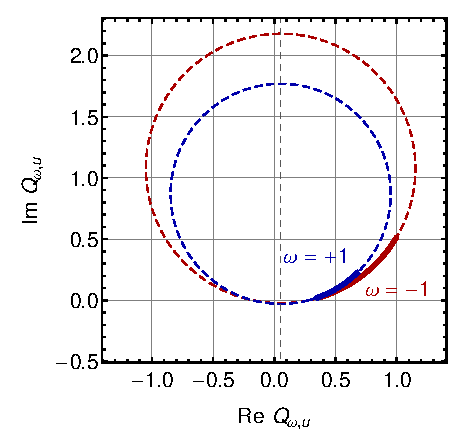
\includegraphics[width=0.8\columnwidth]{vec2s.eps}
\caption{Eigenfunction $Q_{\omega,u}$ for a box spectrum at $\mu=50$. Vertical dashed line contains the centers of the circles.
\label{fig:vec1}}
\end{figure}
%%%%%%%%%%%%%%%%%%%%%%%%%%%%%%%%%%%%%%%%%%%%%%%%%%%%%%%%%%%%%%%%

In Fig.~\ref{fig:vec1} we show the eigenfunctions $Q_{\omega,u}$ for $\epsilon=1/2$ at $\mu=50$.
As remarked earlier,
$Q_{\omega,u}$ is a circular arc in the complex plane for fixed
$\omega$. We have normalized $Q_{\omega,u}$ so that circle centers for different $\omega$ lie on a vertical in the complex plane and the function $Q_{\omega=0,u}$ is a circle of unit radius.
The example in the Fig.~\ref{fig:vec1} is close to the upper instability range, i.e.\ roughly where neutrinos would start converting when the system evolves from high to low $\mu$ values.
In this case the angular modes remain close to each other, corresponding to the observation that the multi-angle system evolves almost like the single-angle one.
%At the onset, the evolution subjects the eigenfunctions to the exponential growth effectively singling them out

%%%%%%%%%%%%%%%%%%%%%%%%%%%%%%%%%%%%%%%%%%%%%%%%%%%%%%%%%%%%%%%%
%\begin{figure}
%\includegraphics[width=0.8\columnwidth]{mat1.eps}
%\caption{Growth rate for continuum, now including matter
%with $\lambda=0$, 10, 100, $10^3$ and $10^4$ (left to right).
%The left-most line ($\lambda=0$) is identical with the ``continuum'' line in
%Fig.~\ref{fig:single1}.
%\label{fig:mat1}}
%\end{figure}
%%%%%%%%%%%%%%%%%%%%%%%%%%%%%%%%%%%%%%%%%%%%%%%%%%%%%%%%%%%%%%%%

%Finally we show in Fig.~\ref{fig:mat1} the instability regions when
%matter is included. In agreement with the previous
%literature~\cite{Banerjee:2011fj, Sarikas:2011am} we find the usual
%multi-angle matter suppression of the instability at low $\mu$
%values. For large matter density, the instability range for $\mu$ is
%shifted to a range around $\mu\sim\lambda$.

\subsection{Normal Hierarchy}

%%%%%%%%%%%%%%%%%%%%%%%%%%%%%%%%%%%%%%%%%%%%%%%%%%%%%%%%%%%%%%%%%
%\begin{figure}
%\includegraphics[width=0.8\columnwidth]{normal_h.eps}
%\caption{Instability parameter $\kappa$ in the case of a normal hierarchy, 
%for $\lambda = 0,\  1,\  1.5,\  2$ (top to bottom).
%\label{fig:normal_h}}
%\end{figure}
%%%%%%%%%%%%%%%%%%%%%%%%%%%%%%%%%%%%%%%%%%%%%%%%%%%%%%%%%%%%%%%%

We next repeat this exercise for the normal hierarchy. In the
single-angle case the system is always stable, a point already known
from the flavor-pendulum~\cite{Hannestad:2006nj}. However, in the
continuum case the system does have instabilities as
predicted in Ref.~\cite{Banerjee:2011fj} based on a simplified
analysis. 
In Fig.~\ref{fig:single1} we show the growth rate as a function of $\mu$ also for the normal hierarchy.
The system is unstable only for a narrow range of
densities with the instability parameter $\kappa$ an order of magnitude lower than in the inverted hierarchy. 

Just as in the inverted hierarchy, including matter suppresses the instability when $\mu\alt\lambda$.
%, i.e.\ when the neutrino density is below the electron density as shown in Fig.~\ref{fig:normal_h}. 
However, in the normal hierarchy we do not observe the shift of the instability towards larger values of $\mu$, resulting in its complete suppression even for small values of $\lambda \sim 1$. 
For a typical SN, at radii where $\mu \sim$ 1--10 km$^{-1}$, the matter potential is usually an order of magnitude higher.
For this reason, collective conversions in the normal hierarchy have not been observed in simulations.

%%%%%%%%%%%%%%%%%%%%%%%%%%%%%%%%%%%%%%%%%%%%%%%%%%%%%%%%%%%%%%%%%%%%%
\section{Discrete Angle Modes}
\label{sec:fewmodes}

\subsection{Eigenvalues and eigenvectors}

If one represents the energy and angle distribution by discrete
bins, the spectrum is implemented as
\begin{equation}
g_{\omega,u}=\sum_{i=1}^{N_\omega}\sum_{j=1}^{N_a}\,
g_{i,j}\,\delta(\omega_i-\omega)\,\delta(u_j-u)\,,
\end{equation}
leading to
\begin{equation}
I_n=\sum_{i=1}^{N_\omega}\sum_{j=1}^{N_a}\,
\frac{u^n_j\mu\,g_{i,j}\,}{\omega_i+u_j\bar\lambda-\Omega}\,.
\end{equation}
One can then determine the eigenvalues $\Omega$ by solving
Eq.~(\ref{eq:multiangleeigenvalue}) which amounts to finding the
roots of an $\Omega$ polynomial of order $N_\omega N_a$.

Alternatively, one can begin with the eigenvalue equation of
Eq.~(\ref{fourier-eom}) in discrete form
\begin{equation}\label{fourier-eom2}
(\omega_k + u_\ell\bar\lambda- \Omega)\, Q_{k,\ell}=
\mu
\sum_{i=1}^{N_\omega}\sum_{j=1}^{N_a}\,
(u_\ell+u_{j})\,g_{i,j}\,Q_{i,j}\,.
\end{equation}
This equation is of the form $(M-\Omega)\,Q=0$ where $Q$ is an
$N_\omega N_a$ dimensional vector of complex numbers and $M$ a
$N_\omega N_a\times N_\omega N_a$ matrix. What remains is to find
the eigenvalues $\Omega$ and eigenvectors $Q_\Omega$ of $M$.
Of course, both methods  provide the same eigenvalues and eigenvectors.
% In explicit examples we find this to be indeed the case.

%%%%%%%%%%%%%%%%%%%%%%%%%%%%%%%%%%%%%%%%%%%%%%%%%%%%%%%%%%%%%%%%
\begin{figure}
\includegraphics[width=0.8\columnwidth]{discrete1a.eps}
\vskip6pt
\includegraphics[width=0.8\columnwidth]{discrete1b.eps}
\vskip6pt
\includegraphics[width=0.8\columnwidth]{discrete1c.eps}
\vskip6pt
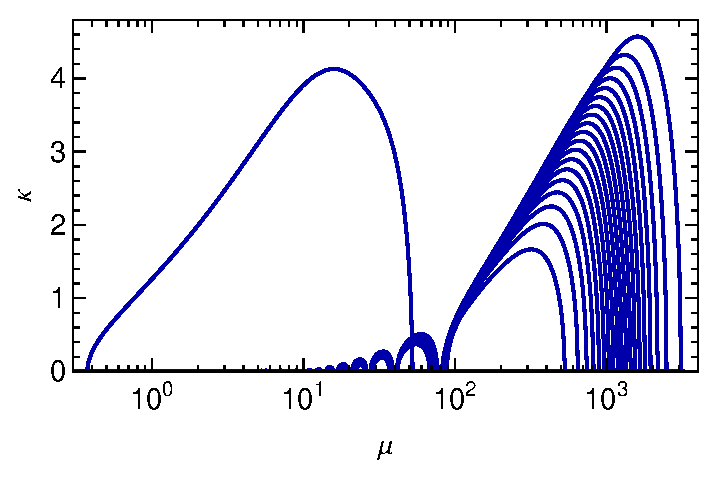
\includegraphics[width=0.8\columnwidth]{discrete1d.eps}
\caption{Growth rates for unstable modes of the hair-comb
spectrum in inverted hierarchy without matter ($\lambda=0$) and $\epsilon=1/2$.
The number of angle modes is
$N_a=2$, 5, 10 and 20 (top to bottom).
\label{fig:discrete1}}
\end{figure}
%%%%%%%%%%%%%%%%%%%%%%%%%%%%%%%%%%%%%%%%%%%%%%%%%%%%%%%%%%%%%%%%
%%%%%%%%%%%%%%%%%%%%%%%%%%%%%%%%%%%%%%%%%%%%%%%%%%%%%%%%%%%%%%%%
\begin{figure}
\includegraphics[width=0.8\columnwidth]{disvec1.eps}
\vskip12pt
\includegraphics[width=0.8\columnwidth]{disvec2.eps}
\caption{Eigenfunctions $Q_{\omega,u}$ for inverted hierarchy
using the hair-comb angle distribution with $N_a=20$, showing
only the $\omega=+1$ case. The discrete locations of the angle modes
are connected by a solid line.
Top: Ordinary mode for $\mu=45$. Bottom: One extra-ordinary mode for
$\mu=1000$.
\label{fig:disvec}}
\end{figure}
%%%%%%%%%%%%%%%%%%%%%%%%%%%%%%%%%%%%%%%%%%%%%%%%%%%%%%%%%%%%%%%%

\subsection{Hair-Comb Spectrum}

We will concentrate on the discrete monochromatic spectrum ($N_\omega=2$) with $N_a$ angle modes representing the original box spectrum:
\begin{equation}
B(u)\to H(u)=\frac{1}{N_a}
\sum_{j=1}^{N_a}\delta\left(\frac{j-1/2}{N_a}-u\right)\,.
\end{equation}
For $N_a=1$ this is our previous single-angle case and for
$N_a\to\infty$ we expect to recover the continuum limit. We can
solve the discrete version of the eigenvalue equation in Mathematica
without problem and show the spectrum of growth rates in
Fig.~\ref{fig:discrete1}.


We always find the ``ordinary mode'' which, for large $N_a$, \marginpar{\footnotesize include continuum limit in the plots?}
approaches the unstable continuum solution. In addition we find
$N_a-1$ ``extra-ordinary modes'' which arise at larger $\mu$. With
increasing $N_a$, the extra-ordinary modes shift their instability
regions to larger $\mu$ values and, in the limit $N_a\to\infty$
disappear at infinity. Of course, for any finite $N_a$, the
extra-ordinary modes exist at a sufficiently large $\mu$.

The presence of the spurious modes is not surprising: solving the eigenvalue equation (\ref{eq:multiangleeigenvalue}) for a discrete case leads to a polynomial of order $2 N_a$ in $\Omega$, whose zeros are eigenvalues. 
It turns out, however, that the discrete $u$-spectrum is just a limiting case of a more general spectral features that cause additional instabilities. We find the upward jump in the $u$-spectrum to be the generic cause of spurious modes. The magnitude ($\kappa$) of this new instability is determined by the gradient of the jump and it's absolute hight, and it's position on the $\mu$-axis by the characteristic $u$-range of the feature in the spectrum.
If the spectrum is zero at first, a possible first jump will not result in new instability.
A descending jump, no matter how steep, does not produce an additional instability. We do not have satisfactory solution for this observation. 

%In this light, we can look at the delta functions of the comb spectrum as infinitely narrow boxes. Each box represents an upward kink in the spectrum 

The different structure of the spurious instabilities can be understood in terms of their eigenfunctions $Q_{\omega,u}$. While for the ordinary mode $Q$'s describe a relatively small arc in the complex plane, reflecting the unison behavior of all angle modes that are locked together, the eigenfunctions of the extra-ordinary modes
%, for the same region of $u\in (0,1)$, 
describe almost the whole circle! The real part of the eigenvalue of spurious modes is always positive $\gamma\sim \epsilon \mu >0$, making possible the resonance of the eigenfunction at $u=(\gamma \pm \omega_0)/\bar\lambda$. The resonance is never possible for the ordinary mode.

For the discrete spectrum, the eigenvectors $Q_{\omega,u}$ are now sets of $N_a$ discrete complex numbers for every $\omega$.
In the upper panel of Fig.~\ref{fig:disvec} we show the ordinary mode for $\mu=45$ and
only for $\omega=+1$. Its structure is similar to the continuous
case. In the bottom panel we show one example of an extra-ordinary
mode which has a completely different arrangement. 
The equidistant grid in $u$ maps very non-linearly to a circle, so that the first and last mode lie close to each other and there is always one mode on resonance, far away from the others. The resonance
width ($\sim \kappa/\bar\lambda$) is approximately the mode spacing, so typically there is
exactly one mode on resonance. The $N_a-1$ extra-ordinary modes
essentially differ by which of the angle modes is on resonance.


%%%%%%%%%%%%%%%%%%%%%%%%%%%%%%%%%%%%%%%%%%%%%%%%%%%%%%%%%%%%%%%%%%%
\section{Origin of the numerical problems in simulations}
\label{sec:simulations}
%%%%%%%%%%%%%%%%%%%%%%%%%%%%%%%%%%%%%%%%%%%%%%%%%%%%%%%%%%%%%%%%%%%

\subsection{Matter suppression}
%%%%%%%%%%%%%%%%%%%%%%%%%%%%%%%%%%%%%%%%%%%%%%%%%%%%%%%%%%%%%%%%
\begin{figure}
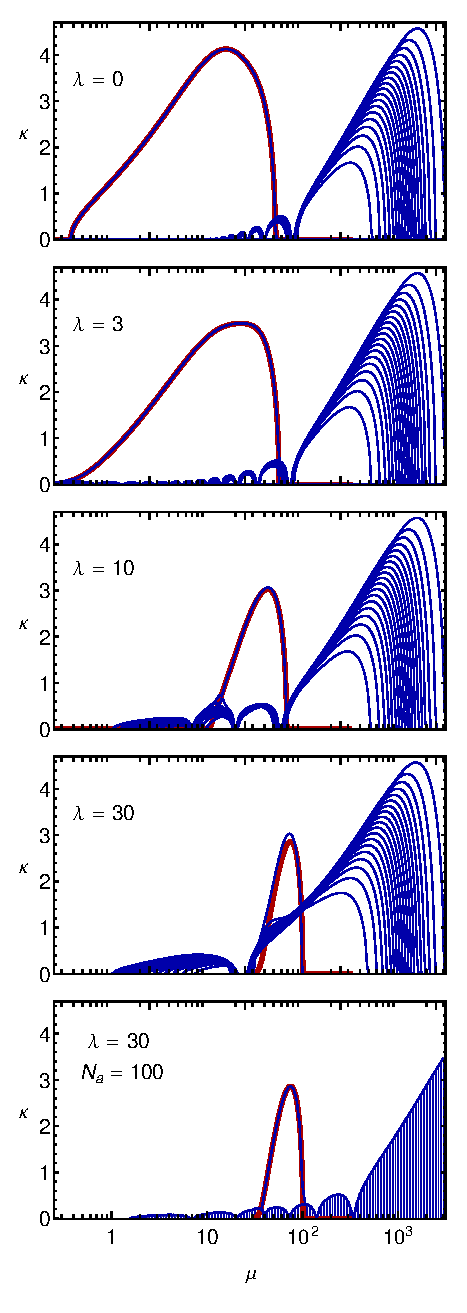
\includegraphics[width=0.8\columnwidth]{discrete_lamda.eps}
\caption{Like Fig.~\ref{fig:discrete1}, for different matter potentials $\lambda=0$, 3, 10, 30. In hatched area in the bottom panel is spanned by the envelope of the spurious modes.
\label{fig:discrete2}}
\end{figure}
%%%%%%%%%%%%%%%%%%%%%%%%%%%%%%%%%%%%%%%%%%%%%%%%%%%%%%%%%%%%%%%%
%%%%%%%%%%%%%%%%%%%%%%%%%%%%%%%%%%%%%%%%%%%%%%%%%%%%%%%%%%%%%%%%
\begin{figure}
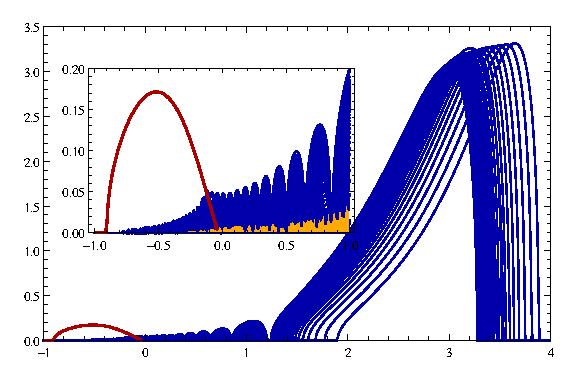
\includegraphics[width=0.8\columnwidth]{realistic_discrete.eps}
\caption{
Growth rate for a realistic SN model ($\epsilon = 0.27$, $\lambda = 3.48 \, \mu^{0.84}$, and $\omega_0 = 0.4$~km$^{-1}$). Thick red line corresponds to the continuum spectrum, blue lines are for a comb spectrum with $N_a=50$ and orange area is the envelope of the spurious modes for $N_a=300$.
\label{fig:discrete2}}
\end{figure}
%%%%%%%%%%%%%%%%%%%%%%%%%%%%%%%%%%%%%%%%%%%%%%%%%%%%%%%%%%%%%%%%

The last ingredient necessary to understand the difficulties of the flavor evolution of SN neutrinos is the effect of the ordinary matter. 
We illustrate our findings in Fig.~\ref{fig:discrete2}.
For the continuum case (thick red line) we confirm the usual
multi-angle matter suppression of the instability at low $\mu$
values, in agreement with the previous
literature~\cite{Banerjee:2011fj, Sarikas:2011am}. For large matter density, the instability range for $\mu$ is
shifted to a range around $\mu\sim\lambda$.

For the comb spectrum (thin blue lines), we find the ordinary mode
expressing the same behavior as the continuum case, as we expected.
The matter, however, does not seem to suppress the spurious instabilities, so with the increase of $\lambda$, the ordinary mode shifts deeper in the region of spurious ones and we lose the clean situation we had in the vacuum case. The only way to again decouple the two regions is to increase the number of angle modes $N_a$. In the example discussed, for $\lambda=30$, we would need $\mathcal{O}(100)$ $u$-modes to be able to integrate safely (Fig.~\ref{fig:discrete2}, bottom panel).


\subsection{Realistic example}

In realistic SN models, the matter potential is not constant, but scales with radius. Typically we $\lambda \propto r^{-m}$, with $m\sim 3.2\text{ to }4$, and $\mu\propto r^{-4}$. In Fig.~\ref{fig:realistic} we show the instability region for an accretion phase SN model, at 300~ms post bounce, described in detail in Refs.~\cite{Chakraborty:2011gd, Sarikas:2011jc}.
Although the physical instability occurs relatively far from the core, we still need high number ($\mathcal{O}(\text{few} 100)$) of angle modes to avoid interference of the spurious instabilities in the system evolution.

\section{Conclusions}

Results of the previous section allow us to finally answer the main questions arising when dealing with numerical simulations: 1) at which radius to start integrating? and 2) how many angle modes to use?

The answer to the first question follows directly from an instability plot $\kappa(r)$ or $\kappa(\mu)$ such as those shown in Figs.~\ref{fig:single1},~\ref{fig:mat1},~\ref{fig:normal_h}.
Our calculation of the onset radius is limited only by the numerical scheme applied to determine the integrals of Eq.~(\ref{eq:In-def}), which is a significant improvement to the simplified analysis of the flavor pendulum \cite{Hannestad:2006nj, Duan:2007mv}.

For the second question, one should simply repeat the instability plot varying the number of angle modes $N_a$ until the maximal growth rate of the extra-ordinary modes below the onset point is at least an order of magnitude lower than the maximal $\kappa$ of the ordinary ones
\begin{equation}
\left.\kern-\nulldelimiterspace
\kappa^{\rm{max}}_{\rm{extra}}(N_a)
\vphantom{\big|}\right|
_{r_{\rm{onset}}} < 
\kappa^{\rm{max}}_{\rm{ord}}\,.
\end{equation}
For instance, in the example shown in Fig.~\ref{fig:discrete1}, $N_a=10$--20 is already enough.

As soon as the integration starts, the dominating growth rate is that of the ordinary mode, leading to the physical solution.
We run a few simulations to confirm this result.
%It is interesting to note that the final outcome of the simulation, for typical parameters in s SN, is not very sensitive to the exact starting point, as long as it is further away from the calculated onset. This feature is not so surprising since the important part is to allow enough time (radius) for the ordinary mode to grow. A few km does not have much effect.
We repeat the counter-intuitive conclusion that by starting a simulation  closer to the SN core does not improve the outcome, but only complicates the study as one integrate through more of the unphysical modes.

%%%%%%%%%%%%%%%%%%%%%%%%%%%%%%%%%%%%%%%%%%%%%%%%%%%%%%%%%%%%%%%%%%%%%%
%\begin{figure}
%\includegraphics[width=0.8\columnwidth]{poly2.eps}
%%\vskip6pt
%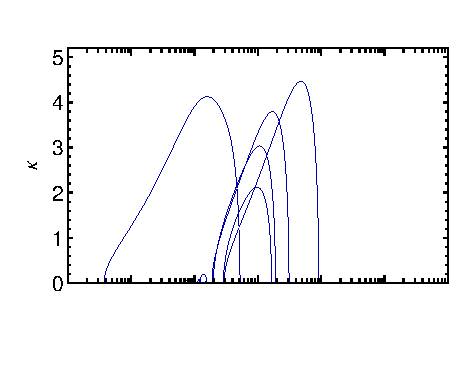
\includegraphics[width=0.8\columnwidth]{poly5.eps}
%%\vskip6pt
%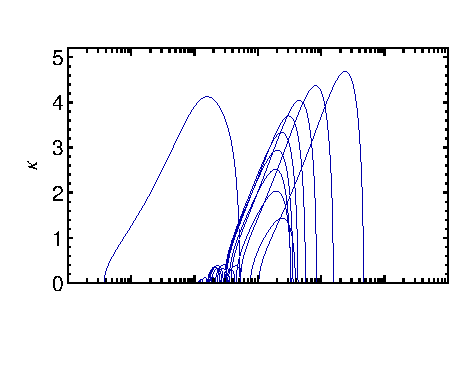
\includegraphics[width=0.8\columnwidth]{poly10.eps}
%%\vskip6pt
%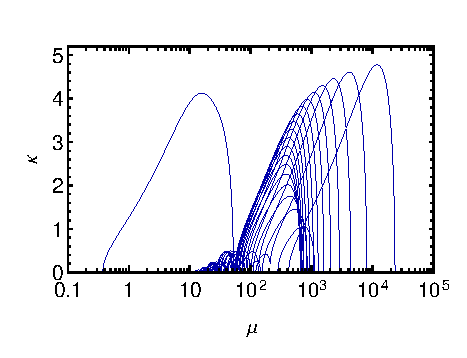
\includegraphics[width=0.8\columnwidth]{poly20.eps}
%\caption{
%Growth rate of polynomial modes fro different truncation order $N_{\rm{trunc}}=2$, 5, 10, 20 (top to bottom).
%\label{fig:polynomials}
%}
%\end{figure}
%%%%%%%%%%%%%%%%%%%%%%%%%%%%%%%%%%%%%%%%%%%%%%%%%%%%%%%%%%%%%%%%%%%%%

%%%%%%%%%%%%%%%%%%%%%%%%%%%%%%%%%%%%%%%%%%%%%%%%%%%%%%%%%%%%%%%%%%%%%%
%\subsection{Polynomial Expansion}
%\label{sec:polynomials}
%%%%%%%%%%%%%%%%%%%%%%%%%%%%%%%%%%%%%%%%%%%%%%%%%%%%%%%%%%%%%%%%%%%%%%

The fact that discretizing a spectrum, necessary for any numerical treatment, leads to the extra-ordinary modes may not be very surprising, and one is tempted to find a smarter way of dealing with the problem, which may present less numerical difficulties. 
Here we show that a projecting the solutions to a space of orthonormal polynomials $p_n(u)$, $u\in [0,1]$ does not solve the problem.


%\clearpage

%%%%%%%%%%%%%%%%%%%%%%%%%%%%%%%%%%%%%%%%%%%%%%%%%%%%%%%%%%%%%%%%%%%%%%
\section*{Acknowledgements} %%%%%%%%%%%%%%%%%%%%%%%%%%%%%%%%%%%%%%%%%%
%%%%%%%%%%%%%%%%%%%%%%%%%%%%%%%%%%%%%%%%%%%%%%%%%%%%%%%%%%%%%%%%%%%%%%

This work was partly supported by the Deutsche
Forschungsgemeinschaft under grant EXC-153 (Cluster of Excellence
``Origin and Structure of the universe'') and by the European Union
under grant PITN-GA-2011-289442 (FP7 Initial Training Network
``Invisibles'').

%%%%%%%%%%%%%%%%%%%%%%%%%%%%%%%%%%%%%%%%%%%%%%%%%%%%%%%%%%%%%%%%%%%%%%
%%%  Bibliography  %%%%%%%%%%%%%%%%%%%%%%%%%%%%%%%%%%%%%%%%%%%%%%%%%%%
%%%%%%%%%%%%%%%%%%%%%%%%%%%%%%%%%%%%%%%%%%%%%%%%%%%%%%%%%%%%%%%%%%%%%%

\begin{thebibliography}{00}

\bibitem{Duan:2006an}
  H.~Duan, G.~M.~Fuller, J.~Carlson and Y.-Z.~Qian,
  %``Simulation of coherent non-linear neutrino flavor transformation in the
  %supernova environment. I: Correlated neutrino trajectories,''
  Phys.\ Rev.\  D {\bf 74}, 105014 (2006).
  %[astro-ph/0606616].
  %%CITATION = PHRVA,D74,105014;%%

\bibitem{Duan:2010bg}
  H.~Duan, G.~M.~Fuller and Y.-Z.~Qian,
  %``Collective neutrino oscillations,''
  Annu.\ Rev.\ Nucl.\ Part.\ Sci.\ {\bf 60}, 569 (2010).
  %%CITATION = ARXIV:1001.2799;%%

%\cite{Duan:2008eb}
\bibitem{Duan:2008eb}
  H.~Duan, G.~M.~Fuller and J.~Carlson,
  %``Simulating nonlinear neutrino flavor evolution,''
  Comput.\ Sci.\ Dis.\  {\bf 1}, 015007 (2008).
  %[arXiv:0803.3650 [astro-ph]].
  %%CITATION = ARXIV:0803.3650;%%

\bibitem{Raffelt:2007cb}
  G.~Raffelt and A.~Yu.~Smirnov,
  %``Self-induced spectral splits in supernova neutrino fluxes,''
  Phys.\ Rev.\  D {\bf 76}, 081301 (2007);
  Erratum ibid.\ {\bf 77}, 029903 (2008).
  %[arXiv:0705.1830];
  %%CITATION = PHRVA,D76,081301;%%
%
%\bibitem{Raffelt:2007xt}
%  G.~Raffelt and A.~Yu.~Smirnov,
  %``Adiabaticity and spectral splits in collective neutrino
  %transformations,''
  Phys.\ Rev.\ D {\bf 76}, 125008 (2007).
  %[arXiv:0709.4641].
  %%CITATION = ARXIV:0709.4641;%%

%\cite{Duan:2007fw}
\bibitem{Duan:2007fw}
  H.~Duan, G.~M.~Fuller and Y.-Z.~Qian,
  %``A simple picture for neutrino flavor transformation in supernovae,''
  Phys.\ Rev.\  D {\bf 76}, 085013 (2007).
  %[arXiv:0706.4293].
  %%CITATION = PHRVA,D76,085013;%%

%\cite{Fogli:2007bk}
\bibitem{Fogli:2007bk}
  G.~L.~Fogli, E.~Lisi, A.~Marrone and A.~Mirizzi,
  %``Collective neutrino flavor transitions in supernovae and the role of
  %trajectory averaging,''
  JCAP {\bf 0712}, 010 (2007).
  %[arXiv:0707.1998].
  %%CITATION = JCAPA,0712,010;%%
%
%\cite{Fogli:2008pt}
%\bibitem{Fogli:2008pt}
  G.~L.~Fogli, E.~Lisi, A.~Marrone, A.~Mirizzi and I.\ Tamborra,
  %``Low-energy spectral features of supernova (anti)neutrinos in inverted
  %hierarchy,''
  Phys.\ Rev.\  D {\bf 78}, 097301 (2008).
  %[arXiv:0808.0807].
  %%CITATION = PHRVA,D78,097301;%%

\bibitem{Dasgupta:2009mg}
  B.~Dasgupta, A.~Dighe, G.~Raffelt and A.\ Yu.\ Smir\-nov,
  %``Multiple spectral splits of supernova neutrinos,''
  Phys.\ Rev.\ Lett.\  {\bf 103}, 051105 (2009).
  %[arXiv:0904.3542].
  %%CITATION = PRLTA,103,051105;%%

\bibitem{Raffelt:2007yz}
  G.~G.~Raffelt and G.~Sigl,
  %``Self-induced decoherence in dense neutrino gases,''
  Phys.\ Rev.\  D {\bf 75}, 083002 (2007).
  %[hep-ph/0701182].
  %%CITATION = PHRVA,D75,083002;%%

%\cite{EstebanPretel:2008ni}
\bibitem{EstebanPretel:2008ni}
  A.~Esteban-Pretel, A.~Mirizzi, S.~Pastor, R.~Tom\`as,
  G.~G.~Raffelt, P.~D.~Serpico and G.~Sigl,
  %``Role of dense matter in collective supernova neutrino transformations,''
  Phys.\ Rev.\  D {\bf 78}, 085012 (2008).
  %[arXiv:0807.0659].
  %%CITATION = PHRVA,D78,085012;%%

%\cite{Raffelt:2008hr}
\bibitem{Raffelt:2008hr}
  G.~G.~Raffelt,
  %``Self-induced parametric resonance in collective neutrino oscillations,''
  Phys.\ Rev.\ D {\bf 78}, 125015 (2008).
  %[arXiv:0810.1407 [hep-ph]].
  %%CITATION = ARXIV:0810.1407;%%

%\cite{Duan:2010bf}
\bibitem{Duan:2010bf}
  H.~Duan and A.~Friedland,
  %``Self-induced suppression of collective neutrino oscillations in a supernova,''
  Phys.\ Rev.\ Lett.\  {\bf 106}, 091101 (2011).
  %[arXiv:1006.2359 [hep-ph]].
  %%CITATION = ARXIV:1006.2359;%%

%\cite{Chakraborty:2011gd}
\bibitem{Chakraborty:2011gd}
  S.~Chakraborty, T.~Fischer, A.~Mirizzi, N.~Saviano and R.~Tom\`as,
  %``Analysis of matter suppression in collective neutrino oscillations during
  %the supernova accretion phase,''
  Phys.\ Rev.\  D {\bf 84}, 025002 (2011);
  %[arXiv:1105.1130].
  %%CITATION = PHRVA,D84,025002;%%
%\cite{Chakraborty:2011nf}
%\bibitem{Chakraborty:2011nf}
  %S.~Chakraborty, T.~Fischer, A.~Mirizzi, N.~Saviano and R.~Tomas,
  %``No collective neutrino flavor conversions during the supernova accretion
  %phase,''
  Phys.\ Rev.\ Lett.\  {\bf 107}, 151101 (2011).
  %[arXiv:1104.4031 [hep-ph]].
  %%CITATION = PRLTA,107,151101;%%
%\cite{Saviano:2012yh}
%\bibitem{Saviano:2012yh}
  N.~Saviano, S.~Chakraborty, T.~Fischer and A.~Mirizzi,
  %``Stability analysis of collective neutrino oscillations in the supernova accretion phase with realistic energy and angle distributions,''
  arXiv:1203.1484.
  %%CITATION = ARXIV:1203.1484;%%

%\cite{Sarikas:2011am}
\bibitem{Sarikas:2011am}
  S.~Sarikas, G.~G.~Raffelt, L.~H\"udepohl and H.-T.~Janka,
  %``Suppression of Self-Induced Flavor Conversion in the Supernova Accretion Phase,''
  Phys.\ Rev.\ Lett.\  {\bf 108}, 061101 (2012).
  %[arXiv:1109.3601 [astro-ph.SR]].
  %%CITATION = ARXIV:1109.3601;%%
%\cite{Sarikas:2012vb}
%\bibitem{Sarikas:2012vb}
  S.~Sarikas, I.~Tamborra, G.~Raffelt, L.~H\"udepohl and H.-T.~Janka,
  %``Supernova neutrino halo and the suppression of self-induced flavor conversion,''
  arXiv: 1204.0971.
  %%CITATION = ARXIV:1204.0971;%%

\bibitem{Hannestad:2006nj}
  S.~Hannestad, G.~Raffelt, G.~Sigl and Y.~Y.~Y.~Wong,
  %``Self-induced conversion in dense neutrino gases:
  %Pendulum in flavor space,''
  Phys.\ Rev.\ D {\bf 74}, 105010 (2006);
  Erratum ibid.\ {\bf 76}, 029901 (2007).
  %[astro-ph/0608695].
  %%CITATION = ASTRO-PH 0608695;%%

%\cite{Duan:2007mv}
\bibitem{Duan:2007mv}
  H.~Duan, G.~M.~Fuller, J.~Carlson and Y.-Z.~Qian,
  %``Analysis of Collective Neutrino Flavor Transformation in Supernovae,''
  Phys.\ Rev.\ D {\bf 75}, 125005 (2007).
  %[astro-ph/0703776].
  %%CITATION = ASTRO-PH/0703776;%%

%\cite{EstebanPretel:2007ec}
\bibitem{EstebanPretel:2007ec}
  A.~Esteban-Pretel, S.~Pastor, R.~Tom\`as, G.~G.~Raffelt and G.~Sigl,
  %``Decoherence in supernova neutrino transformations suppressed by deleptonization,''
  Phys.\ Rev.\ D {\bf 76}, 125018 (2007).
  %[arXiv:0706.2498 [astro-ph]].
  %%CITATION = ARXIV:0706.2498;%%

%\cite{Sawyer:2008zs}
\bibitem{Sawyer:2008zs}
  R.~F.~Sawyer,
  %``The multi-angle instability in dense neutrino systems,''
  Phys.\ Rev.\  D {\bf 79}, 105003 (2009).
  %[arXiv:0803.4319].
  %%CITATION = PHRVA,D79,105003;%%

%\cite{Banerjee:2011fj}
\bibitem{Banerjee:2011fj}
  A.~Banerjee, A.~Dighe and G.~Raffelt,
  %``Linearized flavor-stability analysis of dense neutrino streams,''
  Phys.\ Rev.\ D {\bf 84}, 053013 (2011).
  %[arXiv:1107.2308 [hep-ph]].
  %%CITATION = ARXIV:1107.2308;%%

%\cite{Raffelt:2010za}
\bibitem{Raffelt:2010za}
  G.~G.~Raffelt and I.~Tamborra,
  %``Synchronization versus decoherence of neutrino oscillations at intermediate densities,''
  Phys.\ Rev.\ D {\bf 82}, 125004 (2010).
  %[arXiv:1006.0002 [hep-ph]].
  %%CITATION = ARXIV:1006.0002;%%

%\cite{Raffelt:2011yb}
\bibitem{Raffelt:2011yb}
  G.~G.~Raffelt,
  %``N-mode coherence in collective neutrino oscillations,''
  Phys.\ Rev.\ D {\bf 83}, 105022 (2011).
  %[arXiv:1103.2891 [hep-ph]].
  %%CITATION = ARXIV:1103.2891;%%

\bibitem{Yuzbashyan:2008}
  E.~A.~Yuzbashyan,
  %``Normal and anomalous solitons in the theory of dynamical Cooper
  %pairing,''
  Phys.\ Rev.\ B {\bf 78}, 184507 (2008).
  %%CITATION = PHRVA,B78,184507;%%
  
%\cite{Sarikas:2011jc}
\bibitem{Sarikas:2011jc} 
  S.~Sarikas and G.~Raffelt,
  %``Flavor stability analysis of supernova neutrino fluxes compared with simulations,''
  arXiv:1110.5572 [astro-ph.SR].
  %%CITATION = ARXIV:1110.5572;%%

\end{thebibliography}

\end{document}
